% %%%%%%%%%%%%%%%%%%%%%%%%%%%%%%%%%%%%%%%%%%%%%%%%%%%%%%%%%%%%%%
% This is a template for abstracts for Spring School. Please rename the file according
% to your real surname.
%
% Try not to create much special tex definitions.
%
% The text should be an extended abstract. It will be used as a handout during the
% presentation and then it will be recycled to "Sbornicek" (thin book about Spring
% School). So don't be shy and write more than 10 lines :-)
%
% If you want you may use \section to make sections in the abstract. But try to avoid
% \subsection - We do not have any formating macro for it anyway.
%
% If you wish to use references please do not use \cite and automatic reference
% creation. Instead write directly [1] to the text and create The references by hand.
% Please include references only if they are really important. Do not copy all
% references from an article you are talking about. Note that you do not have to write
% any references to your abstract at all if do not want to.
%
% If you are unsure how the extended abstract should look you may find some
% inspiration in "sbornicek" from recent years, e.g.
% http://kam.mff.cuni.cz/~kamserie/serie/clanky/2006/s773.pdf After reading your
% extended abstract one should understand what is your talk about and have some idea
% what is going on. It is not expected that all proofs will be present.
% 
% If you have any suggestions/comments/patches/hotfixes/dirty jokes please send them
% to Karel: kralka (at) kam.mff.cuni.cz
% 
%%%%%%%%%%%%%%%%%%%%%%%%%%%%%%%%%%%%%%%%%%%%%%%%%%%%%%%%%%%%%
\documentclass[a4paper,10pt]{article}

\usepackage[utf8]{inputenc}
\usepackage{amsmath}
\usepackage{amsfonts}
\usepackage{amssymb}
\usepackage{amsthm}
\usepackage[czech,english]{babel}
\usepackage{fontenc}
\usepackage{bbm}
\usepackage{a4wide} % wider page
\usepackage{hyperref}

\usepackage{graphicx}
\usepackage{float}

\begin{document}

%%%%% Some Macros - leave them as they are  %%%%%
\def\speaker#1#2{                                   
  \centerline{\Large \textbf{#1}}\vskip1pt                
  \centerline{\tt #2} }                                                                          
\def\title#1{\medskip\centerline{\Large \textbf{#1}}}
\def\author#1{\smallskip\centerline{Presented paper by #1}}                                                       
\def\source#1{\smallskip\centerline{(#1)}}
\def\endtitle{\par\medskip}
\newcounter{Defnum}
\newenvironment{definition}{\stepcounter{Defnum}\par\textbf{Definition \arabic{Defnum}.}} {}
\newenvironment{theorem}{\stepcounter{Defnum}\par\textbf{Theorem \arabic{Defnum}.}\it}{}
\newenvironment{lemma}{\stepcounter{Defnum}\par\textbf{Lemma \arabic{Defnum}.}\it}{}
\newenvironment{exercise}{\stepcounter{Defnum}\par\textbf{Exercise \arabic{Defnum}.}\it}{}
\newenvironment{observation}{\stepcounter{Defnum}\par\textbf{Observation \arabic{Defnum}.}\it}{}
\newenvironment{corollary}{\stepcounter{Defnum}\par\textbf{Corollary \arabic{Defnum}.}\it}{}
\newenvironment{conjecture}{\stepcounter{Defnum}\par\textbf{Conjecture \arabic{Defnum}.}\it}{}
\setlength{\parindent}{0pt}
\setlength{\parskip}{0.5 em}
\def\subsection#1{\par Not good idea. \smallskip}
\def\section#1{\par\medskip\centerline{\bf #1}\smallskip}
\def\cite#1{Don't use cite.}
%%%%%% The document itself %%%%%%

\pagenumbering{gobble}

% If you participate in a series please write 
%\title{Ser: How to Irritate People}
% where Ser is:
% HaTu Hanani-Tutte theorem and related topics
% minFPT Minimalist-FPT practitioners course
% Phy Statistical Physics of Optimization Problems
% Or for standalone article:
\title{\protect\parbox{\textwidth}{\protect\centering AlphaGo: Mastering the Game of Go \\ with Deep Neural Networks and Tree Search}}
\author{David Silver, Aja Huang, Demis Hassabis et al. (from Google DeepMind)}% If you present a paper. If not you may skip this
\source{\url{http://www.nature.com/nature/journal/v529/n7587/full/nature16961.html}}

\vskip 1em
Who: Karel Ha (\href{mailto:mathemage@gmail.com}{mathemage@gmail.com}) \\
When: 20\textsuperscript{th} April 2016 (Wednesday), 9:00 - 10:30 \\
Where: S9 \\
Why: Optimization Seminar (NOPT053) \\
\endtitle

\hrule
The game of Go has long been viewed as the most challenging of classic games for artificial intelligence owing to its enormous search space and the difficulty of evaluating board positions and moves.

A~new approach to computer Go introduces \emph{value networks} to evaluate board positions and \emph{policy networks} to select moves.
These deep neural networks are trained by a~novel combination of~supervised learning from human expert games, and reinforcement learning from games of self-play.

Furthermore, a~new search algorithm is introduced: it combines Monte Carlo simulation with value and policy networks.
Using this search algorithm, the computer program AlphaGo developed by~Google DeepMind achieved a~99.8~\% winning rate against other Go programs.

\begin{figure}[H]
  \centering
  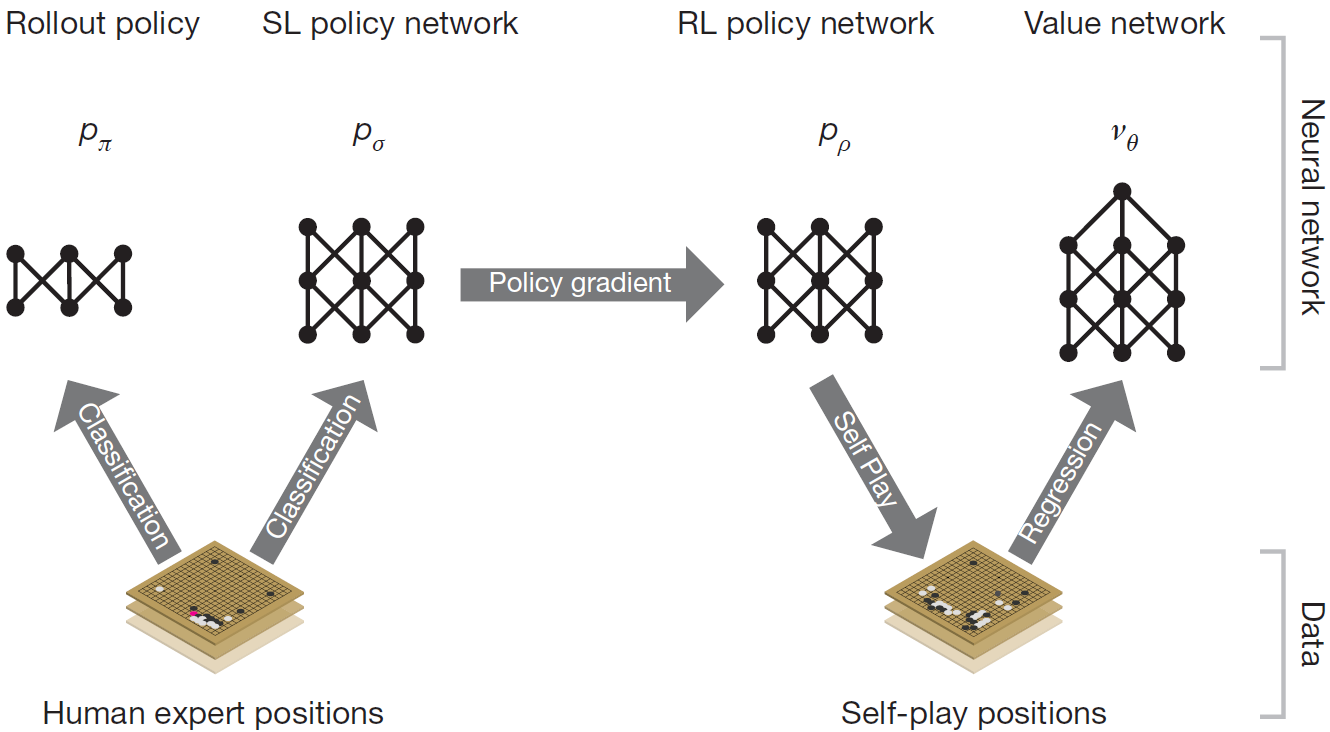
\includegraphics[width=.7\textwidth]{../img/neural_nets_pipeline.png}
\end{figure}
\hrule

\begin{theorem}
  The (distributed version of) AlphaGo plays Go at~the super-human level.
\end{theorem}

\begin{proof}
  The proof is left as an~exercise to the reader.
  The exercise is to~come to~the talk.
  :-)
\end{proof}

\end{document}
